\documentclass[brudnopis]{xmgr}

% \documentclass[openright]{xmgr}

\usepackage{minted}

%\defaultfontfeatures{Scale=MatchLowercase}
%\setmainfont[Numbers=OldStyle,Ligatures=TeX]{Minion Pro}
%\setsansfont[Numbers=OldStyle,Ligatures=TeX]{Myriad Pro}
% for fontspec version < 2.0
% \setmainfont[Numbers=OldStyle,Mapping=tex-text]{Minion Pro}
% \setsansfont[Numbers=OldStyle,Mapping=tex-text]{Myriad Pro}
%\setmonofont[Scale=0.75]{Monaco}

% Opcjonalnie identyfikator dokumentu
% drukowany tylko z włączoną opcją 'brudnopis':
\wersja   {wersja wstępna [\ymdtoday]}

\author   {Krzysztof Sazon}
\nralbumu {243\,696}
\email    {krzysztof.sazon@protonmail.com}

\title    {Zastosowanie modelu Partially Concurrent Open Shop Schedule przy szeregowaniu operacji na danych tabelarycznych}
\date     {2020}
\miejsce  {Gdańsk}

\opiekun  {dr. Hanna Furmańczyk}

% dodatkowe polecenia
%\renewcommand{\filename}[1]{\texttt{#1}}
%\definecolor{stress}{cmyk}{0,1,0.13,0} % RubineRed
%\definecolor{topic}{cmyk}{0.98,0.13,0,0.43} % MidnightBlue

\begin{document}

% streszczenie
\begin{abstract}
W pracy przedstawiono system szeregowania procesów na tabelarycznym zestawie danych w systemie komputerowym oparty o model Partially Concurrent Open Shop Schedule (PCOSS).
Przeanalizowano również jak wydajne (zarówno pod kątem czasu przygotowania jak i pod kątem jakości wyników) są różne heurystyki opisane w pracach innych autorów.
Szczególną uwagę przywiązano do algorytmów opierających się na integralnych czasach przetwarzania bez wywłaszczania.
\end{abstract}

% słowa kluczowe
\keywords{
partially concurrent open shop schedule,
tabular data,
csv,
pandas,
sql}

% tytuł i spis treści
\maketitle

% wstęp
\introduction

W dobie analizy danych...

\section{Oznaczenia przyjęte w pracy}

Hasła "tabla", "tablica", "macierz" stosowane będą zamiennie.

W celu uniknięcia dwuznaczności słowa "procesor" w pracy tratującej o zarówno o modelu matematycznym jak i systemach komputerowych przyjęto używanie słowa "procesor" w rozumieniu pochodzącym z modelu matematycznego (inaczej maszyna).
Procesor w rozumieniu układu scalonego w systemie komputerowym będzie oznaczany anglojęzycznym skrótem, jak CPU czy GPU.

Hasłem "komórka" oznaczony zostanie konkretny, identyfikowalny za pomocą indeksu wiersza i kolumny element tabeli.

\chapter{Pochodzenie modelu Partially Concurrernt Open Shop Schedule (PCOSS) i dotychczasowa literatura}

Model PCOSS został wytworzony przez / w / jako odpowiedź na problem przypisywania techników sprawdzających samolototy w hangarze.
\todo[inline]{itd}

\chapter{Dane tabelaryczne}

Stosowane są one w dziedzinach takich jak analiza statystyczna, prognozowanie trendów czy adaptacja maszyn do środowiska.

\todo[inline]{definicja "tabelaryczne", lub kilka definicji - postrgres, pandas, excel, numpy}
\todo[inline]{przykłady zastosowania - giełda, nauczanie maszynowe, magazyn}

\chapter{Zastosowanie modelu PCOSS do danych tabelarycznych}

W celu uniknięcia dwuznaczności słowa "procesor" w pracy tratującej o zarówno o modelu matematycznym jak i systemach komputerowych przyjęto używanie słowa "procesor" w rozumieniu pochodzącym z modelu matematycznego (inaczej maszyna). Procesor w rozumieniu układu scalonego w systemie komputerowym będzie oznaczany anglojęzycznym skrótem, jak CPU czy GPU.

Praca skupia się na takich sytuacjach, gdy sekwencyjne lub naiwnie zrównolegnienie wykonywanie operacji zajmuje zbyt wiele czasu.

Sytuacje takie występują np. podczas dostępu do danych znajdujących się w zasobach sieciowych, kiedy ograniczeniem jest przepustowość sieci oraz przy dostępie do danych na dysku twardym.

W takim przypadku rolę procesorów z modelu matematycznego przejmują urządzenia (lub ich systemy), takie jak API serwerów sieciowych, procesory (CPU, GPU) czy dyski twarde.
Z kolei role zadań przypadają do kolejnych zestawów wierszy.
Z powyższego wynika bezpośrednio, że operacją staje się praca pewnej instancji pewnego systemu (procesora w rozumieniu wynikającym z modelu) na konkretnym zbiorze kolumn.

W szczególnym (a zarazem najczęstszym przypadku) zestaw wierszy zawiera jeden wiersz, a zestaw kolumn zawiera jedną kolumnę.

\todo[inline]{przykład}

\chapter{Typ danych analizowany w pracy}

W pracy analizowane będą bardzo powszechne operacje na tabelarycznych zestawach danych.
\todo{powtórzenie, więcej konkretów}

W pracy pominięto aspekt zbierania danych jako niezwiązany bezpośrednio z szeregowaniem operacji na nich.

W celu uzyskania oczekiwanych informacji z zestawu danych należy je odpowiednio spreparować a następnie uruchomić narzędzia analityczne na nich.

Wprowadzimy abstrakcję, gdzie zestaw kolumn traktowany jest jako pojedyncza kolumna, a zestaw wierszy jako pojedynczy wiersz.
\todo{rozpisać się na temat, że istnieją przypadki kiedy to ma sens i dlaczego tak robię}


\section{Kreacja danych testowych}

Danymi testowymi będzie lista n krotek o rozmiarze m.
Każda kolejna krotka będzie traktowana jako nowy wiersz, natomiast wszystkie indeksy krotek będą odpowiadały kolumnom. 

\todo{sformułować lepiej, dać matematyczna definicję}

Taki zestaw danych przekłada się na wiele modeli wykorzystywanych w komputerowej analizie danych, jak na przykład tabele czy widoki w relacyjnych bazach danych, DataFrame w Pythonowym pakiecie pandas czy dwuwymiarowa macierz w numpy.
\todo{dodać linki do tych rzeczy}

W rzeczywistym zastosowaniu komórki będą zawierały dane podlegające odpowiednim procesom (obliczeniom), natomiast w danych testowych będą liczbami losowymi, reprezentującymi rozmiar wejścia do funkcji która ma wykonać obliczenia na nich.

\chapter{Algorytm działania dyspozytora}

\section{Wstęp}

W rozumieniu tej pracy dyspozytor to system mający na celu poprawne (wykonalne i zgodne z ograniczeniami) zaszeregowanie i rozdzielanie zadań pomiędzy pomiędzy dostępne procesory.

Wysokopoziomowo algorytm działania dyspozytora opierał będzie się o następujące kroki:

\begin{enumerate}
    \item pobranie danych, ustawienie wartości domyślnych
    \item agregacja danych
    \item przydzielenie szacunkowych czasów wykonania poszczególnych operacji
    \item dobór algorytmu szeregowania 
    \item przygotowanie uszeregowania
    \item czuwanie nad prawidłowym wykonaniem uszeregowania
\end{enumerate}

Każdy z powyższych kroków szczegółowo opisany jest w tym rozdziale.

\newpage
\section{Pobranie danych, ustawienie wartości domyślnych}

Na wejściu algorytm otrzymuje następujące dane wejściowe:

\begin{enumerate}
    \item tabelę w wybranej reprezentacji
    \item listę operacji do wykonania na tabeli
    \item funkcję grupowania wierszy (argument opcjonalny)
    \item funkcję grupowania kolumn (argument opcjonalny)
    \item graf konfliktu (argument opcjonalny)
    \item tabelę złożoności obliczeniowej (zgrupowanych) kolumn (argument opcjonalny)
    \item tabelę czasów przetwarzania (zgrupowanych) kolumn (argument opcjonalny)
    \item algorytm szeregowania (argument opcjonalny)
    \item kryterium optymalizacyjne (argument opcjonalny)
\end{enumerate}

\todo[inline]{dać przykład prawidłowego formatu każdego argumentu}

Tabela \ref{tab:args-default} zawiera domyślne wartości argumentów opcjonalnych \todo{tak często się te nazwy przewijają, że być może warto nadać im symbole}

\begin{table}[!tbh]
\begin{tabular}{|l|l|l|} \hline
Idx. arg. & Wartość domyślna & Interpretacja wartości domyślnej \\ \hline
3 & funkcja identyczności & brak grupowania wierszy \\ \hline
4 & funkcja identyczności & brak grupowania kolumn \\ \hline
5 & graf pusty & wszystkie operacje mogą być wykonywane jednocześnie \\ \hline
6 & nil & algorytm sam ustala złożoność \\ \hline
7 & nil & algorytm sam ustala czasy przetwarzania \\ \hline
8 & nil & algorytm sam dobiera algorytm \\ \hline
9 & $C_{max}$ & kryterium całkowitej długości uszeregowania \\ \hline
\end{tabular}
\caption{Domyślne wartości wejściowe algorytmu i ich interpretacja\label{tab:args-default}}
\source{Własne}
\end{table}

Zagadnienie postępowania algorytmu w zależności od tego, które parametry zostały podane szerzej omówione zostanie w kolejnych podrozdziałach.

\section{Agregacja danych}

W przypadku, gdy podane są funkcje grupowania wierszy i kolumn, algorytm tworzy agregaty zawierające indeksy zakresów zawieranych w tych agregatach.

Tak przygotowane dane gotowe są do przetwarzania w kolejnych etapach działania algorytmu.

\todo[inline]{matematycznie co to agregat, jak to się robi}
\todo[inline]{rozpisać się po co się agreguje w prawdziwym świecie}
\todo[inline]{wstawić pseudokod?}

\newpage
\subsubsection{Przykład}

Przygotowano tabelę wejściową \ref{tab:example-input} w której znajdują się fikcyjne dane na temat sprzedaży produktów M1 i M2 na terenie trzech krajów w dwudniowym okienku czasowym.
Dla tej tabeli przygotowana została agregacja, taka, że kluczem agregacji dla wierszy jest kolumna Kraj (funkcja \ref{eq:example-row-agg}), natomiast z kolumn Sprzedaż$\_$M1 i Sprzedaż$\_$M2 powstaje jedna kolumna z sumą tych wartości (funkcja \ref{eq:example-col-agg}).
Po zastosowaniu funkcji sumy na wierszach wynikowej kolumny należy to interpretować jako sumaryczną sprzedaż wszystkich produktów w całym okresie w danych krajach.

\begin{table}[!tbh]
\begin{tabular}{|l|l|l|l|l|} \hline
Indeks & Kraj & Data & Sprzedaż$\_$M1 & Sprzedaż$\_$M2 \\ \hline
1 & Polska & 01.01.2020 & 7 & 3 \\ \hline
2 & Niemcy & 01.01.2020 & 2 & 6 \\ \hline
3 & Rosja & 01.01.2020 & 5 & 1 \\ \hline
4 & Polska & 02.01.2020 & 2 & 6 \\ \hline
5 & Niemcy & 02.01.2020 & 4 & 2 \\ \hline
6 & Rosja & 02.01.2020 & 17 & 3 \\ \hline
\end{tabular}
\caption{Przykładowa tabela do zagregowania \label{tab:example-input}}
\source{Własne}
\end{table}

Dla przejrzystości funkcji zastosowane zostały skróty

\begin{itemize}
    \item Indeks - $i$
    \item Kraj - $k$
    \item Data - $d$
    \item Sprzedaż$\_$M1 - $s_{m1}$
    \item Sprzedaż$\_$M2 - $s_{m2}$
\end{itemize}

Funkcja agregacji kolumn:
\begin{equation} \label{eq:example-col-agg}
\lambda (i, k, d, s_{m1}, s_{m2}) \\ \Rightarrow (i, k, d, (s_{m1}+s_{m2}))
\end{equation}

Funkcja agregacji wierszy:
\begin{equation} \label{eq:example-row-agg}
\lambda (w_1, w_2, ..., w_{n-1}, w_n) \\ \Rightarrow (w_{g1}, w_{g2}, ..., w_{gm-1}, w_{gm}) 
\end{equation}
gdzie $w_{gx}$ po prawej stronie transformacji, to grupa takich $w_y$ (po lewej stronie), dla których $k$ (kraj) to $x$

Otrzymujemy tabelę wyjściową \ref{tab:example-output}, gotową do obróbki w następnym etapie.

\begin{table}[!tbh]
\begin{tabular}{|l|l|l|l|} \hline
Indeks & Kraj & Dzień & Sprzedaż$\_$M1$\_$Sprzedaż$\_$M2 \\ \hline
(1,4) & Polska & (01.01.2020, 02.01.2020) & (7+3, 2+6) \\ \hline
(2,5) & Niemcy & (01.01.2020, 02.01.2020) & (2+6, 4+2) \\ \hline
(3,6) & Rosja & (01.01.2020, 02.01.2020) & (5+1, 17+3) \\ \hline
\end{tabular}
\caption{Przykładowa tabela po agregacji\label{tab:example-output}}
\source{Własne}
\end{table}

\newpage
\section{Przydzielenie szacunkowych czasów wykonania poszczególnych operacji}

W celu przygotowania poprawnego rozkładu należy znać lub oszacować wartości czasów wykonywania poszczególnych operacji.

Z założeń podanie jednocześnie czasów w postaci argumentów "tabela złożoności obliczeniowej (zgrupowanych) kolumn" oraz "tabela czasów przetwarzania (zgrupowanych) kolumn" jest prawdopodobnie błędem ze strony użytkownika. W takim wypadku zostanie zgłoszony błąd i algorytm przerwie działanie.

Schemat działania przydzielania czasu został przedstawiony na diagramie \ref{diag:time-assign}.

\begin{figure}[!tbh]
\centering
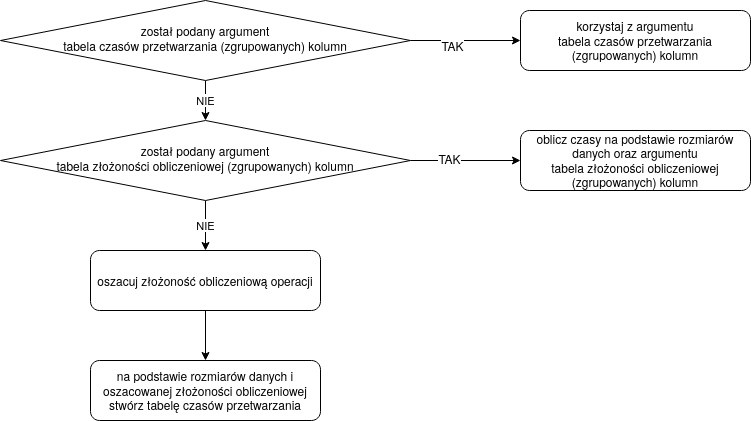
\includegraphics[width=.8\hsize]{fig/przydzielanie_czasow.png}
\caption{Schemat postępowania przy przydzielaniu czasu\label{diag:time-assign}}
\source{Opracowanie własne}
\end{figure}

\subsubsection{Zachowanie algorytmu w zależności od podanych danych na temat czasu}
\todo[inline]{dodać odstęp między tytułem a treścią}

\paragraph{Podano argument "tabela czasów przetwarzania (zgrupowanych) kolumn"}

W przypadku podania poprawnej macierzy czasów operacji ta część algorytmu nie jest wykonywana; zakładamy, że użytkownik podał prawidłowe wartości.
W szczególnym przypadku zadane mogą zostać jednakowe czasy wykonywania operacji.

\paragraph{Podano argument "tabela złożoności obliczeniowej (zgrupowanych) kolumn"}

Ważnym aspektem tego argumentu, jest fakt, że w dziedzinie praktycznej podanie złożoności obliczeniowej nie może ograniczać się do podania samego $O(n)$\todo{rzędu złożoności?} - konieczne jest precyzyjniejsze oszacowanie, wraz ze współczynnikiem oraz składnikiem sumy\todo{wartości dodanej? latencji?}.

Jeżeli na wejściu do algorytmu znajduje się argument "tabela złożoności obliczeniowej (zgrupowanych) kolumn", jedyną operacją która musi zostać wykonana jest podstawienie rozmiarów danych z poszczególnych komórek pod funkcje podane na wejściu.

W szczególnym wypadku użytkownik może podać czasy niezależne od rozmiaru wejścia - na przykład czasy jednostkowe.

\paragraph{Nie podano żadnego z argumentów odnoszących się do czasów przetwarzania}

Na podstawie analizy kilku (np. losowych, lub pierwszych) (zgrupowanych) wierszy algorytm oszacuje złożoność operacji na danym procesorze.
W tym celu zostanie porównany rozmiar wejścia z czasem w którym jest wykonywany, następnie wykorzystując funkcję \emph{curve\_fit} z pakietu \emph{scipy.optimize} zostaną dobrane parametry $a$, $b$, $c$ do funkcji

$$t = f(b * s^a + c)$$

Gdzie $t$ to czas wykonywania, a $s$ to rozmiar danych.
Problem niepokrycia wszystkich możliwych funkcji czasów przetwarzania poruszony został w rozdziale \ref{chap:extend}.

\todo[inline]{być może łatwiej będzie skorzystać z cProfile}
\todo[inline]{napisać to matematycznie}
\todo[inline]{opisać w jaki sposób oceniana jest złożoność funkcji przez curve\_fit}

\section{Dobór algorytmu szeregowania}

\todo[inline]{być może to dobieranie nic ciekawego nie wnosi - seria if-ów}

Jeżeli użytkownik poda obsługiwany przez program algorytm szeregowania, program wykorzysta swoją implementację tego algorytmu.
W przypadku niezaimplementowania wymaganego przez użytkownika algorytmu szeregowania program zgłosi błąd.

Jeżeli algorytm szeregowania nie zostanie podany, to przy zadanym kryterium optymalizacyjnym program dobierze odpowiedni algorytm szeregowania służący do przygotowania optymalnego rozkładu.

Dobór algorytmu polegał będzie na poruszaniu się po drzewie decyzji (bez ingerencji użytkownika).
Wybór podjęty przez rozwiązanie funkcji zwracającej \emph{prawda/fałsz} na każdym poziomu prowadził będzie do kolejnej funkcji w drzewie lub na poziomie liścia - do konkretnego algorytmu.

\section{Przygotowanie uszeregowania}
\todo[inline]{zastosowano uproszczenie: jeden procesor wykonuje tylko jedną funkcję}

Mając przygotowane:

\begin{itemize}
    \item w punkcie "Pobranie i preparacja danych" tabelę wejściową
    \item tabelę czasów z punktu "Przydzielenie szacunkowych czasów wykonania poszczególnych operacji"
    \item graf konfliktu z wejścia
    \item algorytm szeregowania z punktu "Dobór algorytmu szeregowania"
\end{itemize}

można przystąpić do konstrukcji uszeregowania.

Finalny rozkład zostanie przedstawiony w formie tabeli, której indeksy wierszy będą zawierały informacje o planowanym czasie rozpoczęcia wykonania operacji, kolumny przedstawiają procesory natomiast w komórce znajduje indeks wiersz i kolumny zagregowanej tabeli wejściowej (lokalizacja komórki). \todo{matematycznie zapisać}

Przykładowy rozkład wynikowy został przedstawiony w tabeli \ref{tab:example-sched-out}


\begin{table}[!tbh]
\begin{tabular}{|l|l|l|l|l|l|} \hline
Czas & $p_1$ & $p_2$ & ... & $p_{m-1}$ & $p_{m}$ \\ \hline
0 & $[a,b]$ & - & ... & $[c,d]$ & - \\ \hline
2 & - & $[e,f]$ & ... & - & - \\ \hline
5 & $[e,f]$ & $[g,h]$ & ... & - & $[i,j]$\\ \hline
\end{tabular}
\caption{Przykładowe zaszeregowanie wynikowe\label{tab:example-sched-out}}
\source{Własne}
\end{table}


\section{Czuwanie nad prawidłowym wykonaniem rozkładu}

Egzekutor sekwencyjnie czytając wiersze rozkładu zajmował będzie się dysponowaniem operacji w momentach wynikających z indeksu wiersza na odpowiednie procesory.

Idea działania egzekutora została przedstawiona na diagramie \ref{diag:executor}

Istnieje możliwość, w której oszacowanie czasu nie pokryło się z rzeczywistością. Sytuacja została szerzej opisana w rozdziale \ref{chap:extend}

\begin{figure}[!tbh]
\centering
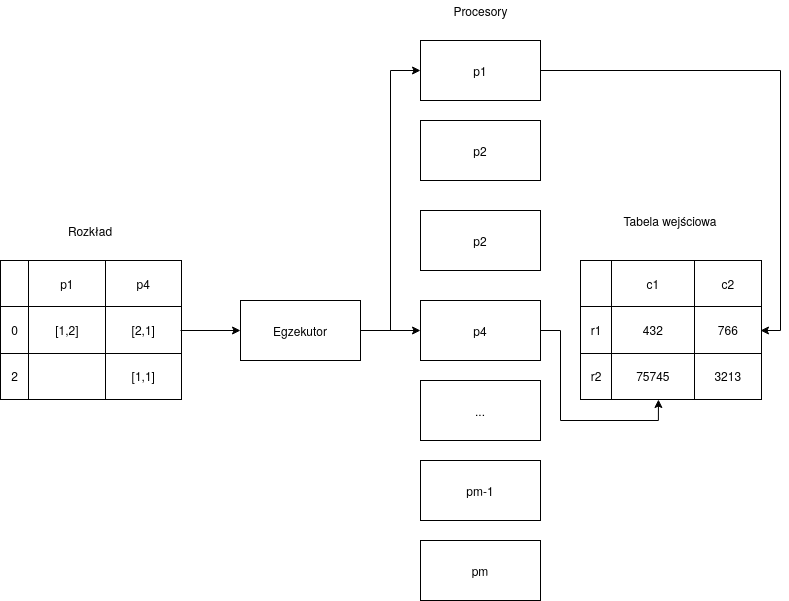
\includegraphics[width=.8\hsize]{fig/executor.png}
\caption{Schemat działania egzekutora\label{diag:executor}}
\source{Opracowanie własne}
\end{figure}



\chapter{Analiza sprawności dyspozytora}


\chapter{Analiza sprawności algorytmów dla podproblemu}


\chapter{Potencjalne kierunki rozwoju pracy} \label{chap:extend}


% zakończenie
\summary

Wszystko poszło pięknie.

% załączniki (opcjonalnie):
\appendix
\chapter{Tytuł załącznika jeden}

Treść załącznika jeden.

\chapter{Tytuł załącznika dwa}

Treść załącznika dwa.

% literatura (obowiązkowo):
\bibliographystyle{unsrt}
\bibliography{xml}

% spis tabel (jeżeli jest potrzebny):
\listoftables

% spis rysunków (jeżeli jest potrzebny):
\listoffigures

\oswiadczenie

\end{document}
